
\chapter{WebTraceCollector}\label{ch:traceCollector}

In order to testing web applications,
we need collects a variety of test cases 
for finding the bugs, analyzing the reasons why the failure happen 
and ensuring the application can work successfully in any circumstances.
However, recording the behaviors on browser manually costs lots of time and work.
It is important to improve the efficiency of web testing by generating test traces automatically.
Thus, we need a tool that can automatically explore web applications and record the traces.

We make a tool named WebTraceCollector that will be introduced in this chapter for automatically generating traces of Websites.
WebTraceCollector is wrote on Python 3 and using Selenium as Library.
It can open a browser with selenium and explore the Website with the browser automatically.
Depending on the Document Object Model\cite{DOM} of the current web page,it will find the suitable clickable elements to click.
WebTraceCollector can also work fine on the dynamic websites with Ajax\cite{ajax} application,
and insert texts into every input text fields with the fitting data.

%為了測試APP和WEB,our lab使用了一些工具來產生traces
%this paper 用python 和 seleium為基底建立一個可以自動explore website的trace collector
%此工具用DOM tree來做state-base的finite state machine

\clearpage

\section{Framework}

There are several kinds of work,
such as taking snapshot, inserting values and deciding the next element to click, during the web testing.
To manage all works, WebTraceCollector collects all events by a list.
It also constructs a finite state machine to record every web page in the website 
and represent the link between web pages by the edges and states.
The framework of WebTraceCollector is shown in Fig \ref{collectorFramework}.

At the first step of testing, WebTraceCollector go to the target URL and start to recognize the first web page.
The web page will be converted into a state of a finite state machine.
In order to explore the website deeper,
the clickable elements and input fields should be identified and 
the next action event depending on the clickable elements will be added into the event list.
WebTraceCollector constantly get an event from the list
and implement a event at once until the list is empty.

After implementing an action, WebTraceCollector will check the status of the webpage.
If the web page changes, the new web page will be converted into a new state and saved in the automata.
Similarly, the clickable elements of new web page should be identified and 
the events of new clickables will be added into event list.

The algorithm of WebTraceCollector is shwon in algorithm \ref{AutomataOverview}.

\begin{algorithm}[htb]
	\begin{doublespace}		
		\KwIn{ URL, algo }
		Initial(URL)\;
		Current\_State $\gets$ Web\_Page\;
		Automata.add\_state( State )\;
				
		\While{ Event\_List $\neq$ Empty }
		{
			Event $\gets$ Event\_List.Get\_Event()\;
			Do\_Event( Event )\;
			Next\_State $\gets$ Web\_Page\;
			\If{ Next\_State $\neq$ Current\_State  }
			{
				Automata.add\_state( Next\_State )\;
				Event\_List.Add\_Event( Next\_State )\;
			}
			Current\_State $\gets$ Next\_State\;
		}		
	\end{doublespace}
	\caption{Overview}
	\label{algorithm:overview}
\end{algorithm} 

\begin{figure}[h]
\graphicspath{{pic/}}
\begin{center}
	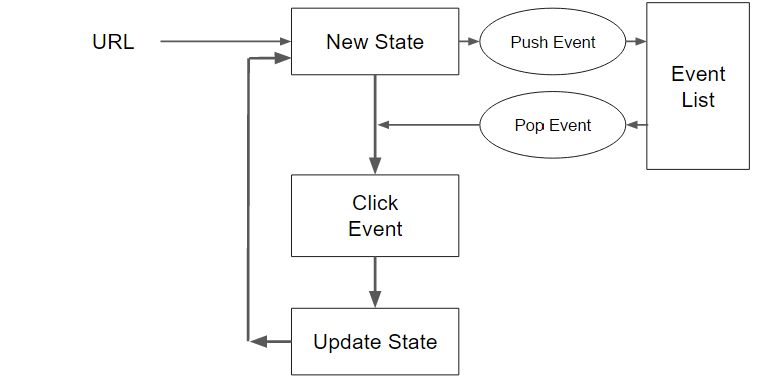
\includegraphics[width=0.8\textwidth]{collectorFramework.png}
\end{center}
\caption{The framework of WebTraceCollector. }
\label{collectorFramework}
\end{figure}

%此工具一邊使用selenium來操縱web browser,
%一邊建立state(DOM), edge(click ,inputs) 的automata
%此工具使用event list的形式,選擇一個algorithm,每次pop out一個待辦的event
%每次update:若是新的state,就將所有的clickables排入events,若是舊的state就無視

\clearpage

\section{Webpage identification}

WebTraceCollector record the current page of the browser into a state in the finite state machine.
In order to identify a web page,
we distinguish the web pages according to the DOM tree.
The DOM tree is the tree structure of the web elements.
However, we can not directly access the DOM tree of the web page by the browser,
the method to solve this problem is downloading the page source of web page by selenium 
and rebuild the DOM tree by the library BeautifulSoup\cite{BS4}.

After building the DOM tree, the elements in the web page are known.
The clickable elements are defined as <a> tag, <button> tag and <input> tag with button attribute. 
WebTraceCollector find all the clickable elements in the DOM tree
and convert them into event objects.
The events will be added into event list,
so the testing will continue to click these element later.

In some complex case, the website is not only work by the simple buttons 
but also javascript functions that have bind mouse listener on other elements.
It is almost impossible to guess which element have the javascript function,
becuase we only do black box testing of the web applications 
and we do not know how the web applications work 
for understanding the javascript code in the web page is too difficult.
Even so, most of the web applications still can tested by this method,
and automated testing still saves lots of human effort.

\clearpage

\section{Event}

During the testing, WebTraceCollector repeats getting an event from the event list 
and implements the action of the event until the event list is empty.
The procedure of event is shown in Fig \ref{ClickEvent}.
An event consists of action, state and depth.
The action implies which clickable element should be clicked.
The state implies where web page the element locates in.
The depth implies how deep this event is in the automata.
Every event has only one action, which means it only click one button at one time.
According to the DOM tree of the web page, the clicking action will insert the value into the input fields.

Before the event start, 
WebTraceCollector checks the current state on the browser.
Because if the current state is not equal to the state recorded on the event,
the wrong element will be clicked and the change of the state will be recorded and lead to wrong automata.
If the current state is not equal to the state on the event, 
it should change the web page to where the clickable element locates.
Most of the time, it can reached by trace back history from the browser.
But in the case of complex website ,it will be hard to retrun the correct web page.
In that case, the automata find the simple past from the initial state of wepsite to the target state,
and WebTraceCollector will go through the simple path to reach the target web page.

Once the arrive to the correct web page, WebTraceCollector will start to clicke the target element.
However, web pages not only have clickable elements,
the dynamic web pages also have input fields need to insert and 
lead to different reaction according to the value that user inserted.
To work fine on those dynamic websites that not only have buttons to click but also have other input fields,
WebTraceCollector needs to insert values into those elements when it implements the clicking action.
The input field elements are defined as <input> tag, <select> tag, <radio> tag and <checkbox> tag.
Because the Website may only accept certain words as input values likes, 
we can not just make random string to test the Website.
we construct a database to analysis the element and find the most suitable string.
The database has some example values of the common inputs we generalize from websites.
Considering the element's tag, id, name and other siblings tags,
WebTraceCollector will use the most similar string to the examples as the input value of the element.
The algorithm of implementing the action is shwon in algorithm[\ref{algorithm:action}].

\begin{algorithm}[htb]
	\begin{doublespace}		
		\KwIn{ action, state, depth }
		\If{ Current\_State $\neq$ state }
		{
			Back\_Track( state )\;
		}
		Clickable $\gets$ action.Get\_Clickable()\;
		Inputs, Selects, Radios, Checkboxes $\gets$ state.getFormElements()\;
		\ForEach{ Element in Inputs, Selects, Radios, Checkboxes }
		{
			Value $\gets$ Database.Find\_Value( Element )\;
			Set\_Value( Element, Value )\;
		}
		Click\_Clickable()\;		
	\end{doublespace}
	\caption{To implement the action}
	\label{algorithm:action}
\end{algorithm} 


\begin{figure}[h]
	\graphicspath{{pic/}}
	\begin{center}
		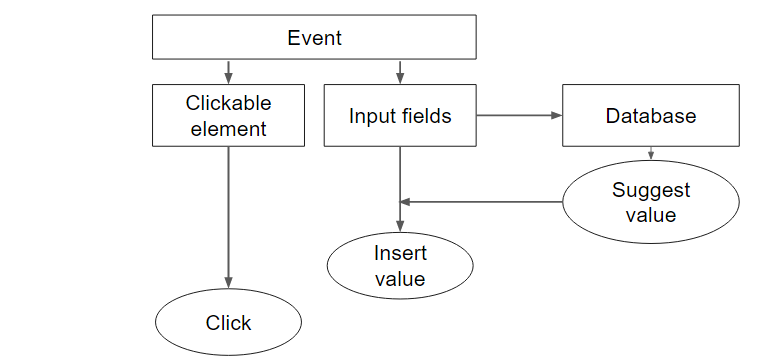
\includegraphics[width=0.8\textwidth]{ClickEvent.png}
	\end{center}
	\caption{The  procedure of click event. }
	\label{ClickEvent}
\end{figure}

%要執行click action時,會先對所有的input 填值,會連上database進行input,clickable的tag等feature的字串處理,找出推薦的適當的值填入

\clearpage

\section{Suggested value}

The problem of guessing the correct value of specific input field is very difficult.
Because we only implement the black box testing, it is hard to realize the meaning of the current web page
while unknowing the whole codes of the web applications.
The method we can use is analyzing the text of the element 
and trying to guess the meaning of the input element.

We constrcut a database which storing lots of example values of common input elements.
A partial of the database is shown in Table \ref{InputDatabase}.
Each data is an example value of a common feature 
and each feature has several normalized keywords.
For example, a feature email has keywords "email" and "信箱" and some exmple valuse like "Ann@gmail.com".
For a specific input element,
we analyze the element's tag name, id attribute, name attribute and text.
If the attributes of the elements similar to the keywords of a feature,
we will suggest that the feature is suitable to be the value of the input element.
Then, one of the examples randomly selected and insert into the input field.

While an event is implementing, WebTraceCollector not only choose the target clickable element
but also need to insert the suitable value into every input fields on the web page.
Those input fields' detailed infomation will analyzed with the database 
and the sugested value will generated by string analysis.


\begin{table}[ht]
	\begin{center}
		\begin{tabular}{ | l | l | l | l | }
			\hline
			Feature & value 1 & value 2 & value 3 \\ \hline
			email / 信箱 & Ann@hotmail.com.twn & Bob@gmail.comn & Cindy@yahooo.com \\ \hline
			name / 名字 & Ann & Bob & Cindy \\ \hline
			job / 職業 & studentn & engineern & officer \\ \hline
			gender / 性別 & man & woman & \\ \hline
			phone / 電話 & 0900123456n & 0987654321n & 0911001011 \\ \hline
			address / 地址 & \#12 abc street & 5 floor \#12 sun street & \# USA   \\
			                & Tainan Taiwan  &  Pintung Taiwa         & orange,2323 \\ \hline
			birth / 生日 & 2001/02/03 & 1999/04/03 & 1988/11/30 \\ \hline			
		\end{tabular}
		\caption{ Part of the input database. }
		\label{InputDatabase}
	\end{center}
\end{table}

\section{Normalization}

After the action, WebTraceCollector will check what happens on the browser 
by comparing the current state of the web page and other states in the automata.
The state objects have the information of DOM tree loading from the browser by Selenium.
If the DOM tree is same after click event, the clickable element will be regarded as ineffective and no edge and reaction will happen.
On the other hand, if the DOM tree changes, the clickable element will be regarded as effective link.
The clickable and the input values will made as a edge and added into automata.

However, there are some problems if we just regard the two DOM trees as strings and compare.
For example, there may be advertising applications, calenders, popularity numbers or catalogs shown on the website.
Each time user visits the website, the DOM tree of the website may be different.
To prevent recognizing a wrong state, we must preprocess the DOM tree.

The work of preprocessing is removing the elements that may confuse us and remain the elements we want to focus on.
We remove the tags that are unvisible on the web page, the javascripts code, the HEAD of the html and the css style.
We construct a class named normalizer, which can scan the DOM tree, find the target element and remove it.
For specific website, User can set the specific normalizer to normalize the DOM tree by his own style.
The examples of DOM tree and normalized DOM tree are shown in Fig[\ref{DOMvsNorDOM}].

%state用DOM比較,但有問題需要省略
%省略的方式有config

\begin{figure}[h]
	\graphicspath{{pic/}}
	\begin{center}
		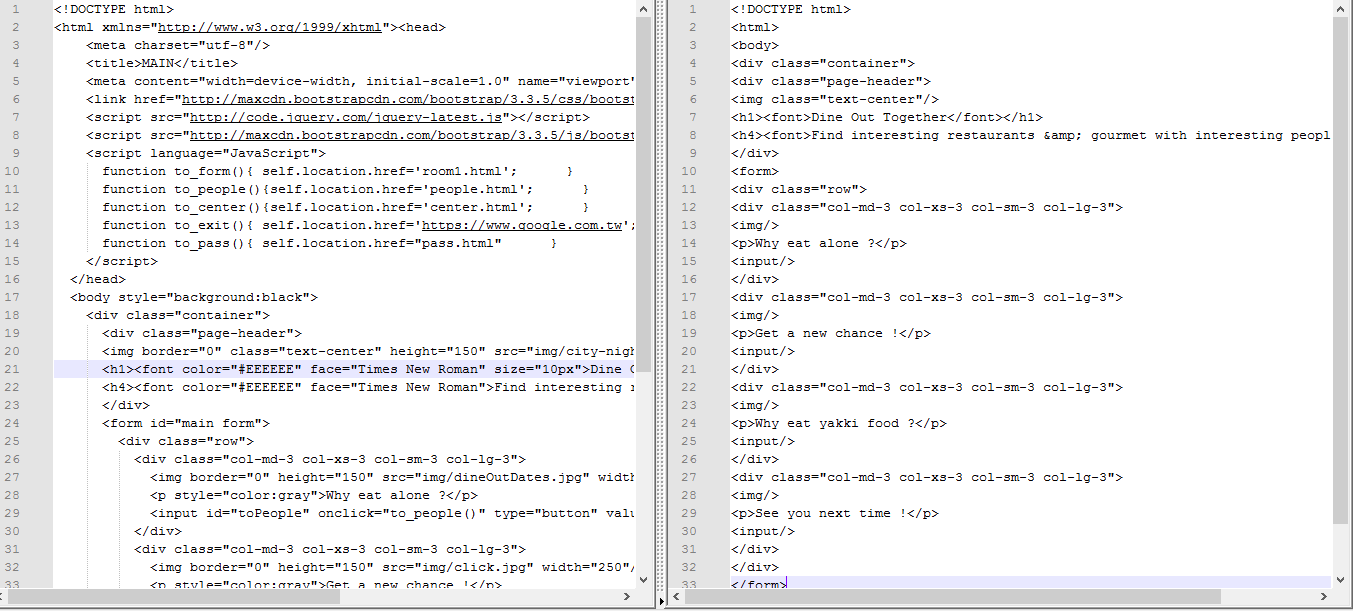
\includegraphics[width=0.8\textwidth]{DOMvsNorDOM.png}
	\end{center}
	\caption{An Example of DOM tree compare with Normalize DOM tree. }
	\label{DOMvsNorDOM}
\end{figure}

\clearpage

\section{Automata and traces}

We construct an finite state automata, which consists of states and edges, to represent the Website
with each state represent a web page and each edge represent the link from one web page to another.
The state is defined based on the DOM tree of the web page.
If the URL, DOM tree or any element on the web page changes, we will recognize that it goes to other state.
The edge records one state goes to another state by an action,
which clicks the specific clickable tag with values written in all form elements.

In order to view the automata clearly and help user to understand the automata easily,
WebTraceCollector generate a HTML file to show the graph of the automata.
In the html, every state represented by the snapshot of the web page,
and every edge between two states are represented by the arrows connected between the two states.
The example web page of automata is shown in Fig[\ref{AutomataOverview}].

As the test result, WebTraceCollector generates traces information in different types of files. 
There are JSON files of traces and automata, screenshots of every state, DOM tree and detail information of every state and a web page of overview automata.
Automata.json records all states, which have URL, ID, screenshot and DOM tree of the web page, and edges.
Traces.json records the states and edges with the order
The example of the test result is shown in Fig[\ref{TestResult}].

\clearpage

\begin{figure}[h]
	\graphicspath{{pic/}}
	\begin{center}
		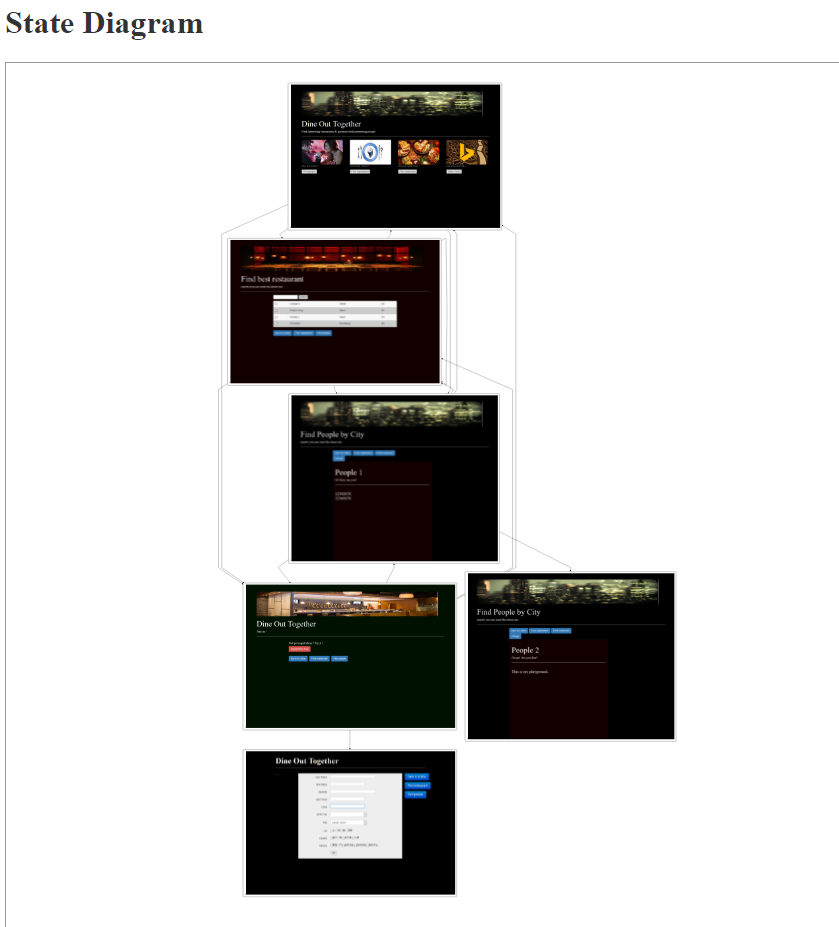
\includegraphics[width=0.6\textwidth]{automata_overview.png}
	\end{center}
	\caption{ Overview of the Automata. }
	\label{AutomataOverview}
\end{figure}

\begin{figure}[h]
	\graphicspath{{pic/}}
	\begin{center}
		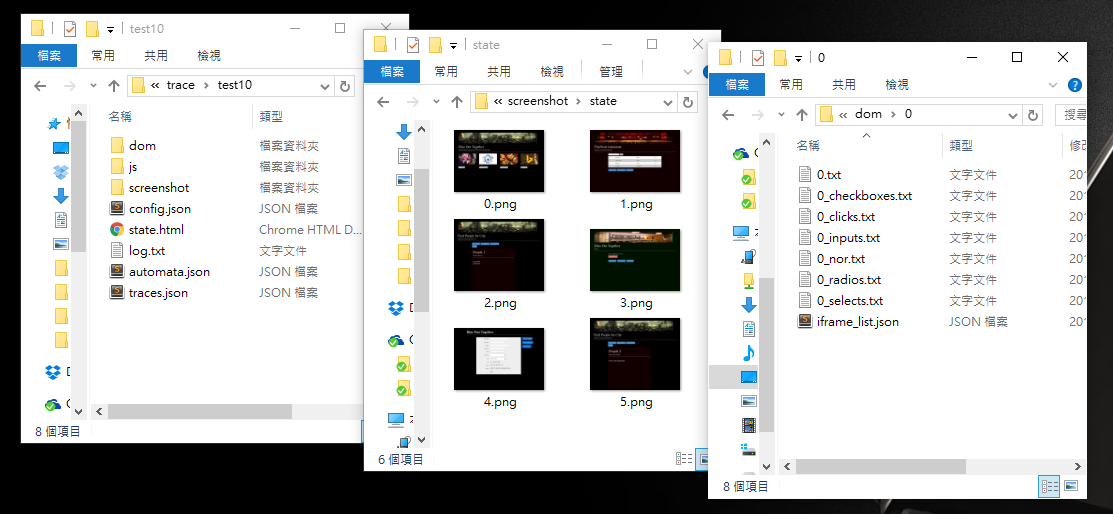
\includegraphics[width=0.8\textwidth]{webTraceResult.png}
	\end{center}
	\caption{An Example traces of the website. }
	\label{TestResult}
\end{figure}

%一個element:有clickable,input,radio,checkbox,select
%一個state:有ID,dom list,all elements,all clickable
%其中DOM又含有iframe的結構
%一個edge:有ID,from to state,all elements with value,one clickable
%一個trace:有states edges照order排

\clearpage

\section{Trace collection}

WebTraceCollector can explore the website with algorithm set by user.
We make two algorithms for WebTraceCollector: Monkey and DFS.
User can choose the algorithm and set to the config as an input before starting the test.
WebTraceCollector will switch it's reaction by the algorithm at every stage after action during the test.

%根據不同的algorithm,此工具面對可按的clickables

\subsection{Monkey}

The monkey algorithm simply adds a random event to the event list.
Every time when WebTraceCollector detects the DOM tree changed and encounters a different state,
it collects all clickable elements from the current state and randomly choose one as next event.
User can set the trace length and trace amount in the config,
which means the maximum edges in one trace and the total amount of all traces.
The trace generated by monkey algorithm may contains a loop, 
because monkey algorithm may choose the same clickable.

%每次update:在length max以前,在現在state可見的clickables中隨機挑一個排入events

\subsection{Depth First Search}

The disadvantage of monkey algorithm is that it may only visit certain web pages and not explore the whole website.
To guarantee all clickable elements will be clicked durring the testing,
We develop the DFS algorithm.
However, Some Websites is too huge to explore all of it's web pages, like Wiki or News,
or too complicated that makes unlimited different web pages, like chat room or other dynamic websites. 
User need to set the maximum depth of the DFS,
so the DFS algorithm only explore the website with the depth from the initial web page less than the max depth.

Unlike the Monkey algorithm, DFS algorithm adds all evenst on the current state to the event list.
When WebTraceCollector encounter a different web page,
it will download the page source of the web page as a state and compare the current state with other states in the automata.
For the four different situations mentioned before,
the DFS algorithm has different reaction.
If the current state is a new state, which means this web page does not visited before,
this state will added into the automata and all clickable elements will made as an event and added into the event list.
If the currenrt state is an old state or is as same as the last state,
there will be no new events added and continue next event.
If the URL is out of the domain, WebTraceCollector will ignore this state and back to the last state.

\clearpage

